\section{Database}
Per facilitare l'identificazione delle entità coinvolte nel database si è utilizzato un modello entità-relazione che fornisce una rappresentazione grafica chiara e intuitiva della struttura dei dati. Questo modello aiuta a visualizzare le entità (oggetti o concetti del mondo reale), le relazioni (le associazioni tra le entità) e gli attributi (le proprietà o le caratteristiche delle entità e delle relazioni).
\subsection{Modello Entità-Relazione}
Nel seguente diagramma entità-relazione in Figura~\ref{fig:er_diagram}, osserviamo che le comande possono essere costituite da più ordini effettuati dai clienti. Tali clienti sono suddivisi in due categorie: clienti d’asporto identificati tramite numero di telefono e clienti al tavolo identificati tramite numero del tavolo. I piatti, consultabili tramite un menù, sono caratterizzati da un ingrediente principale. Una volta ordinato un piatto dal menù, questo viene inserito al’interno di un ordine identificato da un codice progressivo per cliente, e viene successivamente inserito nella comanda del rispettivo cliente. La comanda sarà quindi utilizzata per identificare il cliente e contiene i piatti ordinati oltre che il totale dello scontrino con il corrispettivo codice di pagamento.

\begin{figure}[H]
	\centering
	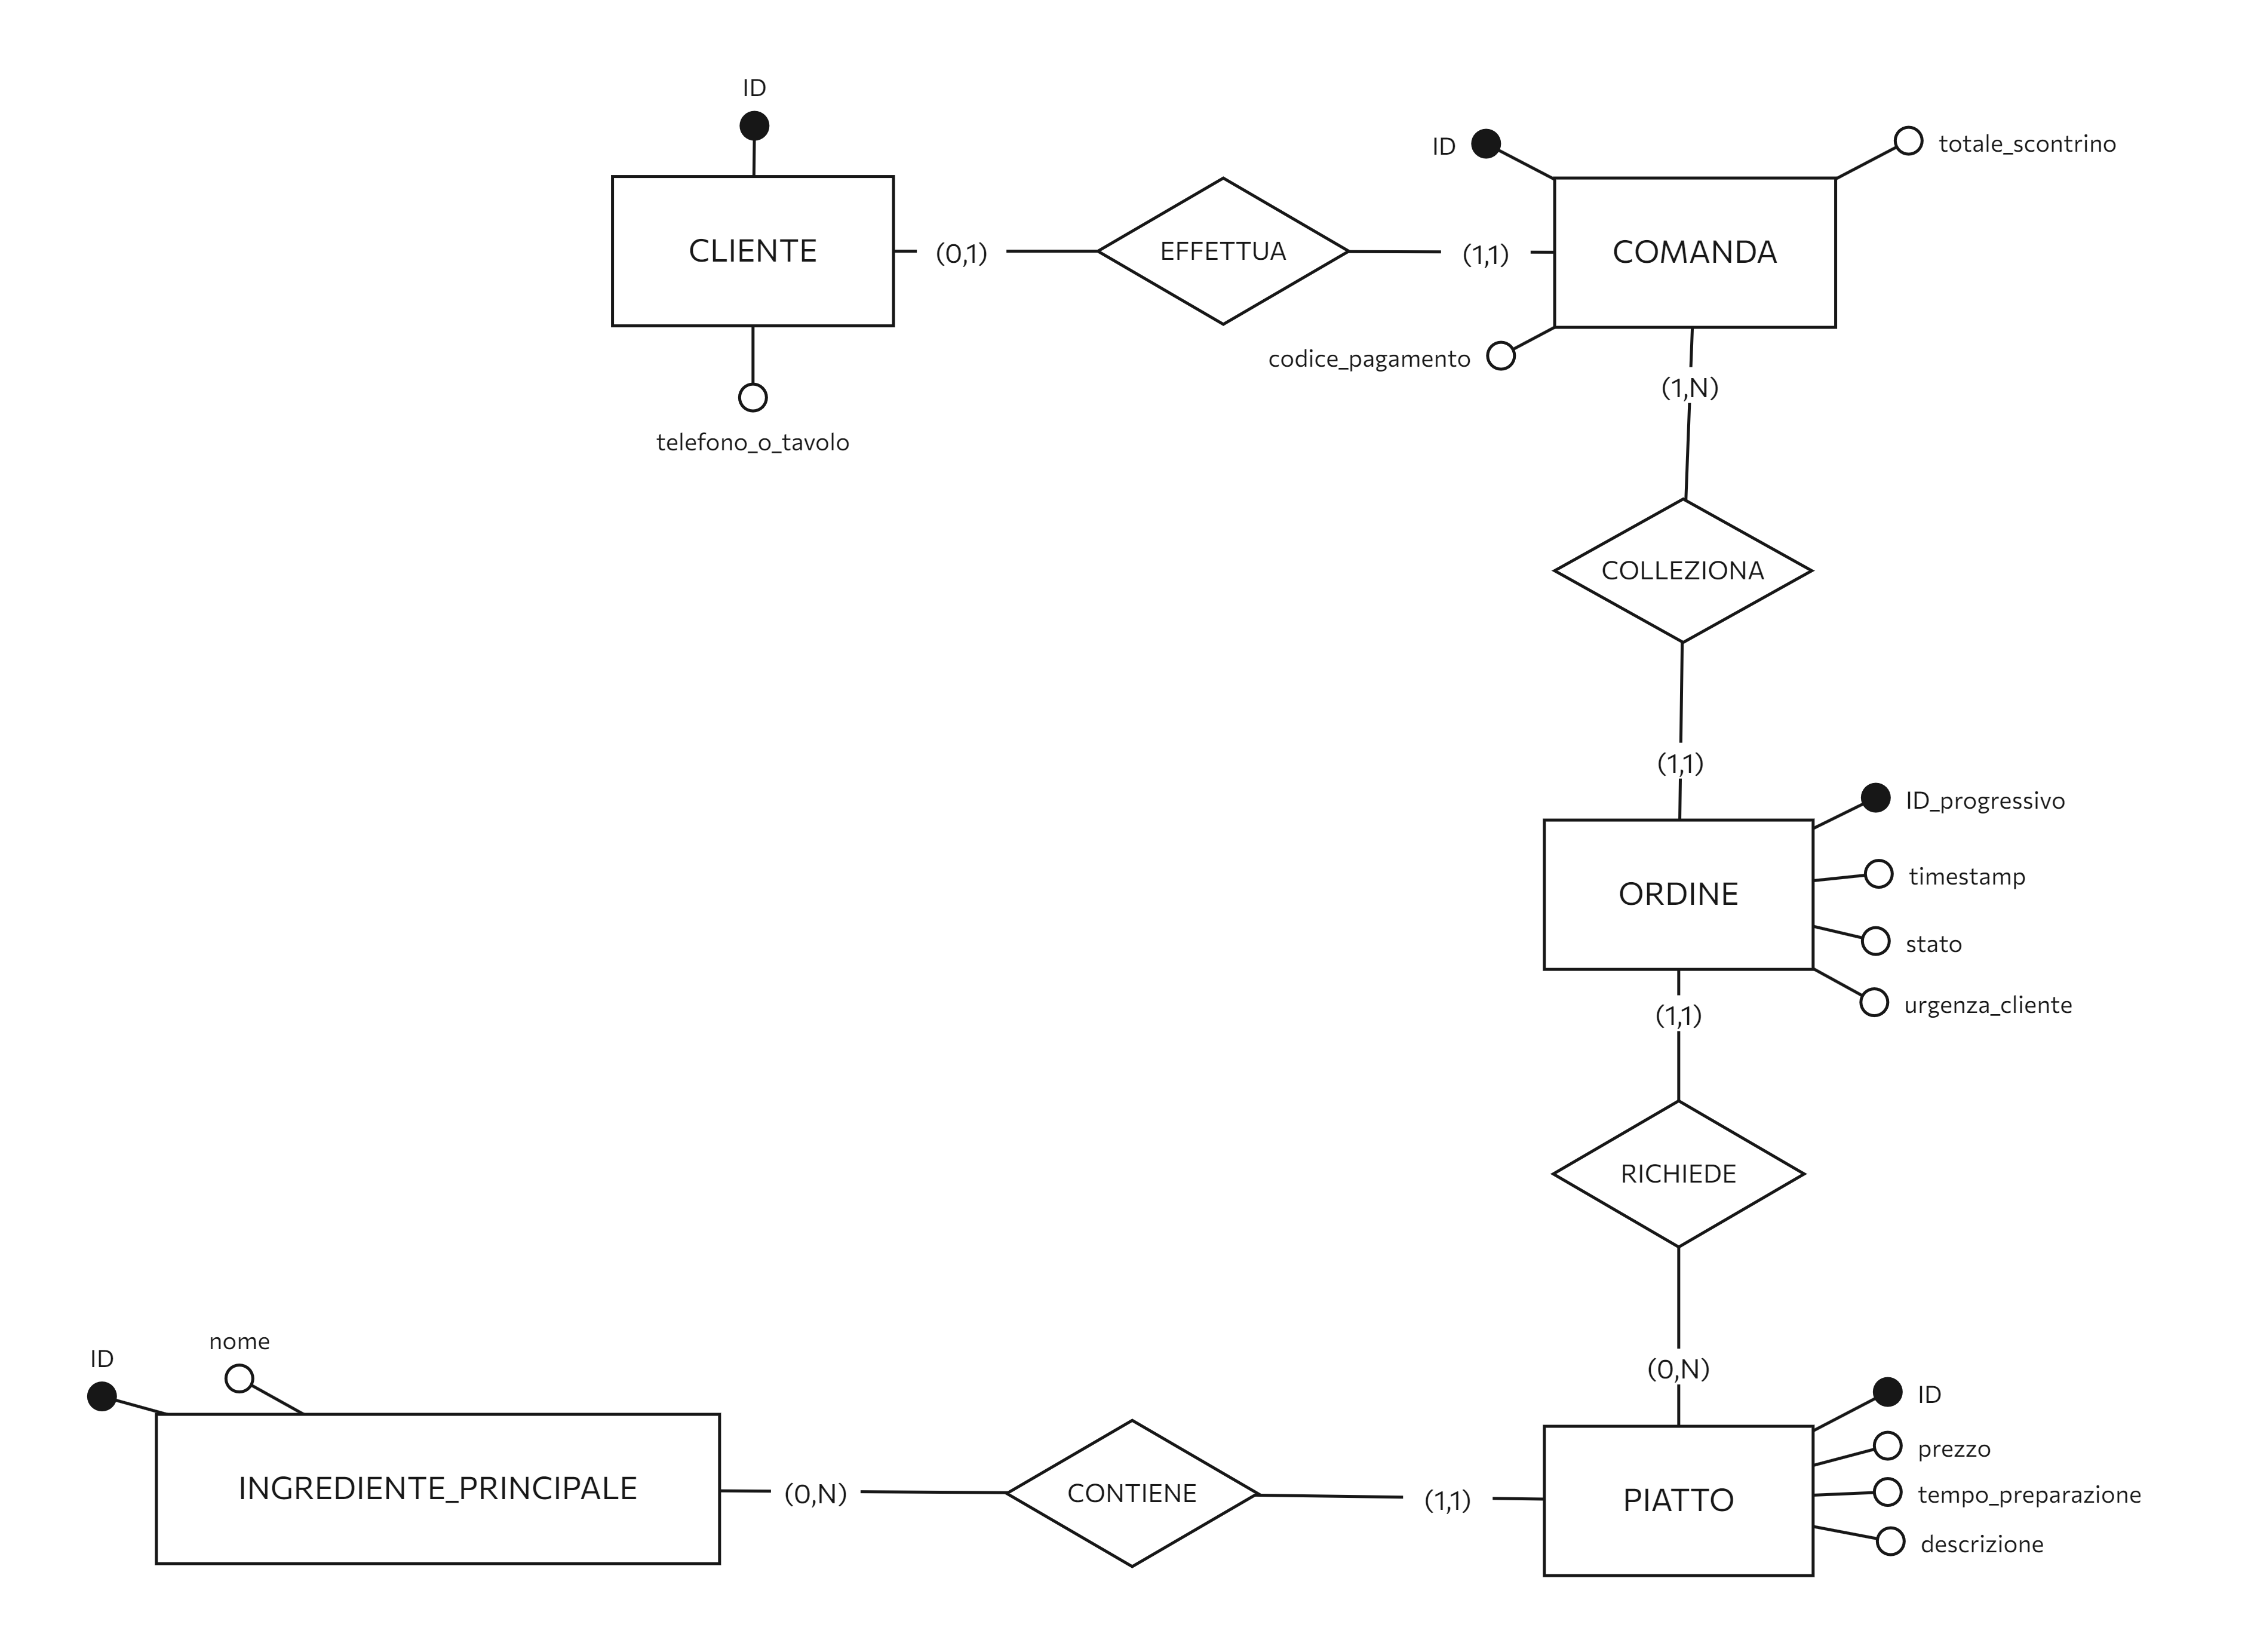
\includegraphics[scale=0.4]{iterazione1/images/ER_project_c.png}
	\caption{Modello Entità-relazione\label{fig:er_diagram}}
\end{figure}

\subsection{Modello logico}
Tramite il modello logico viene rappresentata in modo astratto la struttura dei dati così da facilitare la progettazione del database, definendo come i dati sono organizzati e come le entità interagiscono tra loro.
Rappresentazione della struttura dei dati all’interno del database. L’attributo di cliente::asporto\_o\_tavolo è stato pensato come un boolean in quanto il cliente può essere di due tipi:
\begin{itemize}
	\item se asporto\_o\_tavolo = 0, allora l’ID sarà il codice identificativo di un tavolo;
	\item se asporto\_o\_tavolo = 1, allora l’ID sarà un numero di telefono;
\end{itemize}

\begin{figure}[htbp]
	\centering
	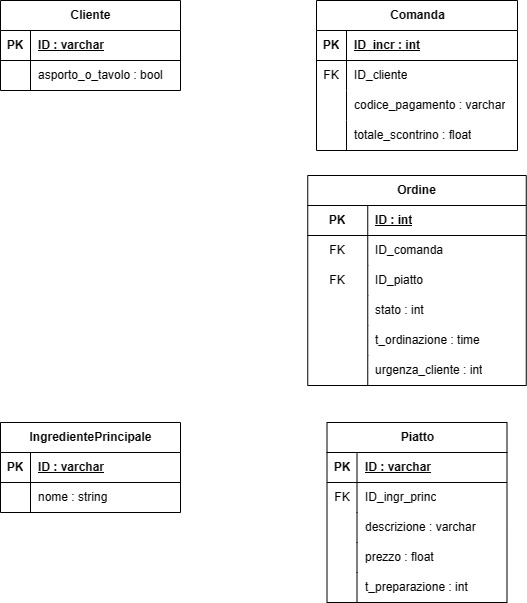
\includegraphics[scale=0.5]{iterazione1/images/database_modello_logico.jpg}
	\caption{Modello Logico\label{fig:modello_logico}}
\end{figure}

\newpage
Il modello logico è implementato con le seguenti query al database:

\begin{lstlisting}[language=SQL,caption=Query del database in SQL,label=lst:sqlcode]
CREATE TABLE IF NOT EXISTS Cliente(
    ID varchar(10) PRIMARY KEY,
    t_o_a boolean NOT NULL
);

CREATE TABLE IF NOT EXISTS Comanda (
    ID int(10) AUTO_INCREMENT,
    ID_cliente varchar(10) NOT NULL,
    codice_pagamento varchar(255) DEFAULT NULL,
    totale_scontrino float DEFAULT 0.0,
    PRIMARY KEY (ID),
    FOREIGN KEY (ID_cliente) REFERENCES Cliente(ID)
);

CREATE TABLE IF NOT EXISTS IngredientePrincipale(
    ID varchar(20) primary key,
    nome varchar(20) not NULL
);

CREATE TABLE IF NOT EXISTS Piatto(
    ID varchar(20) NOT NULL PRIMARY KEY,
    ID_ingr_princ varchar(20) NOT NULL,
    descrizione varchar(50),
    prezzo float(6) NOT NULL,
    t_preparazione int,
    FOREIGN KEY (ID_ingr_princ) REFERENCES IngredientePrincipale(ID)
);

CREATE TABLE IF NOT EXISTS Ordine(
    ID int(10) NOT NULL AUTO_INCREMENT PRIMARY KEY,
    ID_comanda int(10) NOT NULL,
    ID_piatto varchar(20) NOT NULL,
    stato int(1) DEFAULT 0, -- 0=creato, 1=in coda, 2=in preparazione, 3=completato
    t_ordinazione TIMESTAMP DEFAULT CURRENT_TIMESTAMP,
    urgenza_cliente int(2) DEFAULT 0, -- priorità del cliente: 1=massima, -1=minima
    FOREIGN KEY (ID_comanda) REFERENCES Comanda(ID),
    FOREIGN KEY (ID_piatto) REFERENCES Piatto(ID),
    CHECK (stato >= 0 AND stato <= 3 )
);
\end{lstlisting}

\clearpage